\chapter{Magnetismo de sólidos} \label{Ch:10}

En este Capítulo se estudian algunas de las contribuciones más importantes al magnetismo de los sólidos. Como se verá, alguna de ellas (como la ferromagnética) constituye un fenómeno cooperativo que lleva asociado una transición de fase. Es también destacable que el magnetismo de sólidos es en buena medida un efecto cuántico dado que muchas de sus causas (el momento mangnético de espín, la interacción de intercambio, etc.) no tienen análogo clásico.

\section{Relaciones básicas}

La \textbf{magnetización} (o imanación) $\Mn$ se define como el momento magnético por unidad de volumen 

\begin{equation}
	\Mn = \frac{1}{V} \sum_V \mun	
\end{equation}
donde los $\mun$ son los momentos magnéticos atómicos o iónicos en el ``volumen de control'' $V$. Recordemos que para partículas sin espín $\mun =  \sum_i \frac{1}{2} \rn_i \times q_i \vn_i$ y que para \textit{lazos} de corriente $\mun  = I \An$ siendo $I$ la intensidad y  $\An$ el área encerrada. El magnetismo de los sólidos se clasifica de acuerdo a la interrelación de su magnetización con el campo magnético aplicado $\Hn$. Así, se introduce la \textit{susceptibilidad magnética} $\chi$ por 

\begin{equation}
	\Mn = \chi \Hn
\end{equation}
En general $\chi$ será un tensor, pero no consideraremos esta complicación aquí. Si un medio tiene $\chi$ negativa se el sólido se dice \textit{diamagnético} y si por contra $\chi$ es positiva el sólido se dice \textit{paramagnético}. Además, existe un grupo de materiales que pueden poseer magnetización aun en ausencia de campo aplicado y que son \textit{ferromangéticos} (observar que $\chi \rightarrow \infty$).

\section{Diamagnetismo atómico}

La naturaleza del diamagnetismo atómico se puede comprender a partir de un modelo clásico en que cada órbita electrónica es considerada una espira de corriente. De acuerdo con la ley de Lenz, al variar el flujo magnético sobre el circuito surge una fuerza electromotriz de inducción que hace variar la corriente y por tanto genera un momento magnético adicional. Así, si $A$ es el área de la órbita, $\omega$ la velocidad angular e $I$ la intensidad de corriente, el momento magnético será $\mu=IA=-(e\omega / 2\pi)A$, y bajo la aplicación de un campo $B$ perpendicular a la órbita, aquél se incrementa en

\begin{equation}
	\Delta \mu = - \frac{eA}{2\pi} \Delta \Omega \label{Ec:10-02-01}
\end{equation}
La variación de velocidad angular $\Delta \omega$ se determina del balance de fuerzas sobre la órbita, que consideramos circular de radio $r$ (ver figura \ref{Fig:10-01}): antes de la aplicación del campo de fuerza nuclear se equipara a la fuerza centrífuga, $F_\text{núcleo} = m\omega^2 r$; tras la aplicación del campo aparece adicionalmente la fuerza de Lorentz $F_L = ev B$ dirigida hacia el núcleo, que se compensa con un aumento de la velocidad angular 

\begin{equation}
	m(\omega + \Delta \omega)^2 r = F_\text{núcleo} + e v B
\end{equation}
Como para los campos magnéticos aplicables en un laboratorio $evB\ll m \omega^2 r$, se tiene que $\Delta \omega \ll \omega$. Así pues, despreciando términos en $\Delta \omega^2$ se deduce 

\begin{equation}
	\Delta \omega = \frac{evB}{2mr\omega} = \frac{eB}{2m}
\end{equation}
que se denomina \textit{frecuencia de Larmor}. Combinando con (\ref{Ec:10-02-01}) y generalizando a un átomo de $Z$ electrones:

\begin{equation}
	\Delta \mu = - Z \frac{e^2A}{4\pi m} B = - Z \frac{e^2 \langle \rho^2 \rangle}{4m}B
\end{equation}
siendo $\langle \rho^2 \rangle = \langle x^2 + y^2 \rangle = \langle x^2 \rangle + \langle y^2 \rangle$ el valor cuadrático medio de la distancia de los electrones al eje que pasa por el núcleo paralelamente al campo (eje $z$). Si admitimos simetría esférica, $\langle x^2 \rangle=\langle y^2 \rangle=\langle z^2 \rangle$ y con ello el radio cuadrático medio atómico resulta $\langle r^2 \rangle\= \frac{3}{2} \langle \rho^2 \rangle$. Llamando $n$ al número de átomos por unidad de volumen la magnetización resultante es

\begin{equation}
	M = n \Delta \mu = - \frac{nZe^2 \langle r^2 \rangle}{6m}B
\end{equation}
y la susceptibilidad magnética 

\begin{equation}
	\chi = \frac{M}{H} \approx \frac{mu_0 M}{B} = - \frac{\mu_0 n Z e^2 \langle r^2 \rangle}{6m}
\end{equation}
que es el resultado clásico de \textit{Langevin}. Aunque en general $B=\mu_0 (H+M)$, aquí se ha aproximado $B\approx \mu_0 H$ dado que $|M|\ll H$ (o bien que $|\chi |\ll 1$). En efecto, para $n=5\times10^{28} \unit{m}^{-3}$ y $r=10^{-10}$ m, $\chi = -10^{-6}Z$. El diamagnetismo atómico es propio de \textit{todos los cuerpos sin excepción}, aunque a menudo está enmascarado por el paramagnetismo o el ferromagnetismo.



\begin{figure}[h!] \centering
	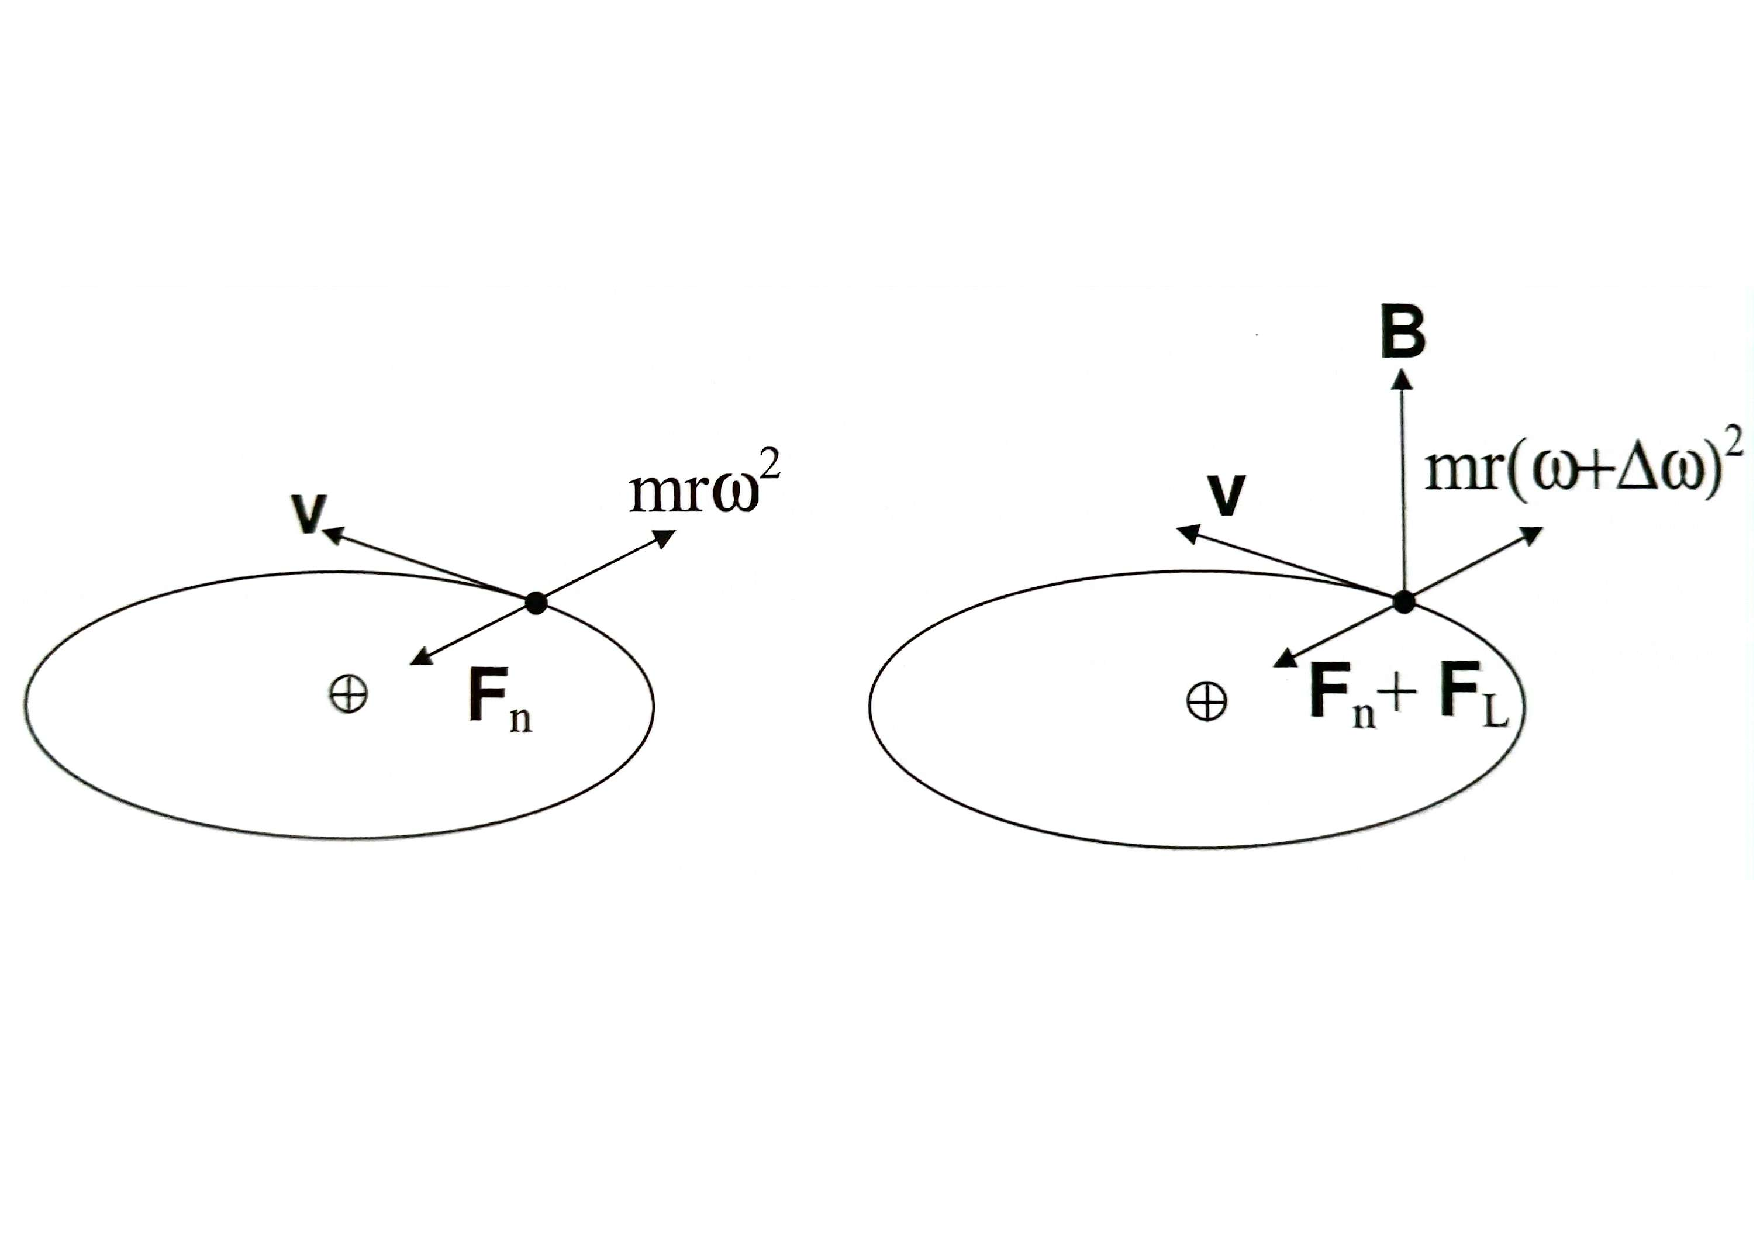
\includegraphics[scale=0.35]{Cuerpo/Ch_10/Fotos libro 1.pdf}
	\caption{Balance  de fuerzassobre un electrón orbitando en torno a un núcleo en ausencia (izquierda) o en presencia (derecha) de un campo mangético externo. El referencial usado es uno centrado en el núcleo y que gira con el electrón de modo qeu hay que considerar las fuerzas inerciales (aquí sólo hay fuerza centrífuga).}
	\label{Fig:10-01}
\end{figure}

\section{Paramagnetismo atómico}

\subsection{Origen del momento mangnético atómico}

\subsection[Dependencia de la magnetización respecto $\vec{\Bn}$ y $T$]{Dependencia de la magneteización paramagnética con la temperatura y el campo magnético}

\subsection{Ley de Curie}

\section{Paramagnetismo de los electrones de conducción}

\section{La interacción de intercambio}

\section{Ferromagnetismo}

\section{Dominios ferromagnéticos}

\section{Orden ferrimangnético}

\begin{figure}[h!] \centering
	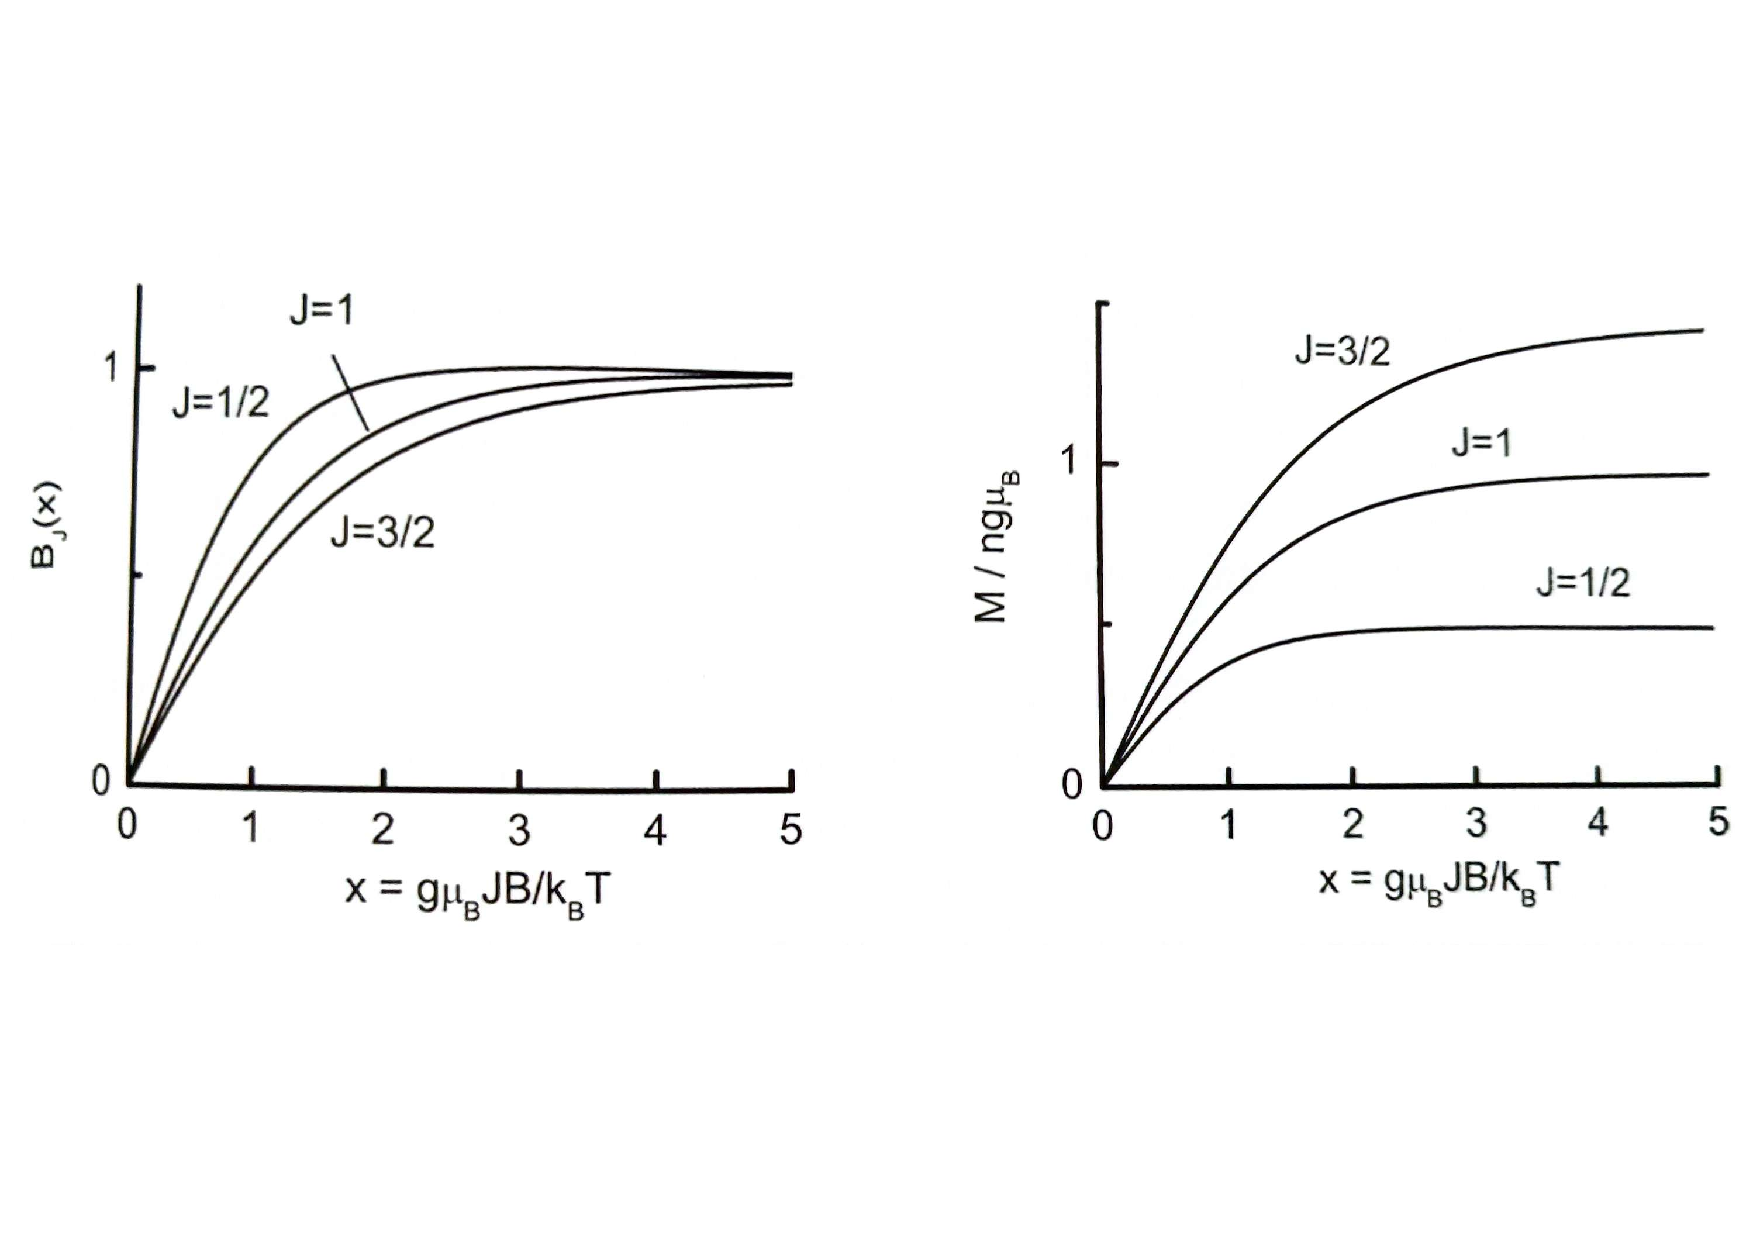
\includegraphics[scale=0.35]{Cuerpo/Ch_10/Fotos libro 2.pdf}
	\caption{Dependencia con $x$ de la función de Brillouin y de la magnetización paramagnética para distintos valores de $J$.}
	\label{Fig:10-02}
\end{figure}
\begin{figure}[h!] \centering
	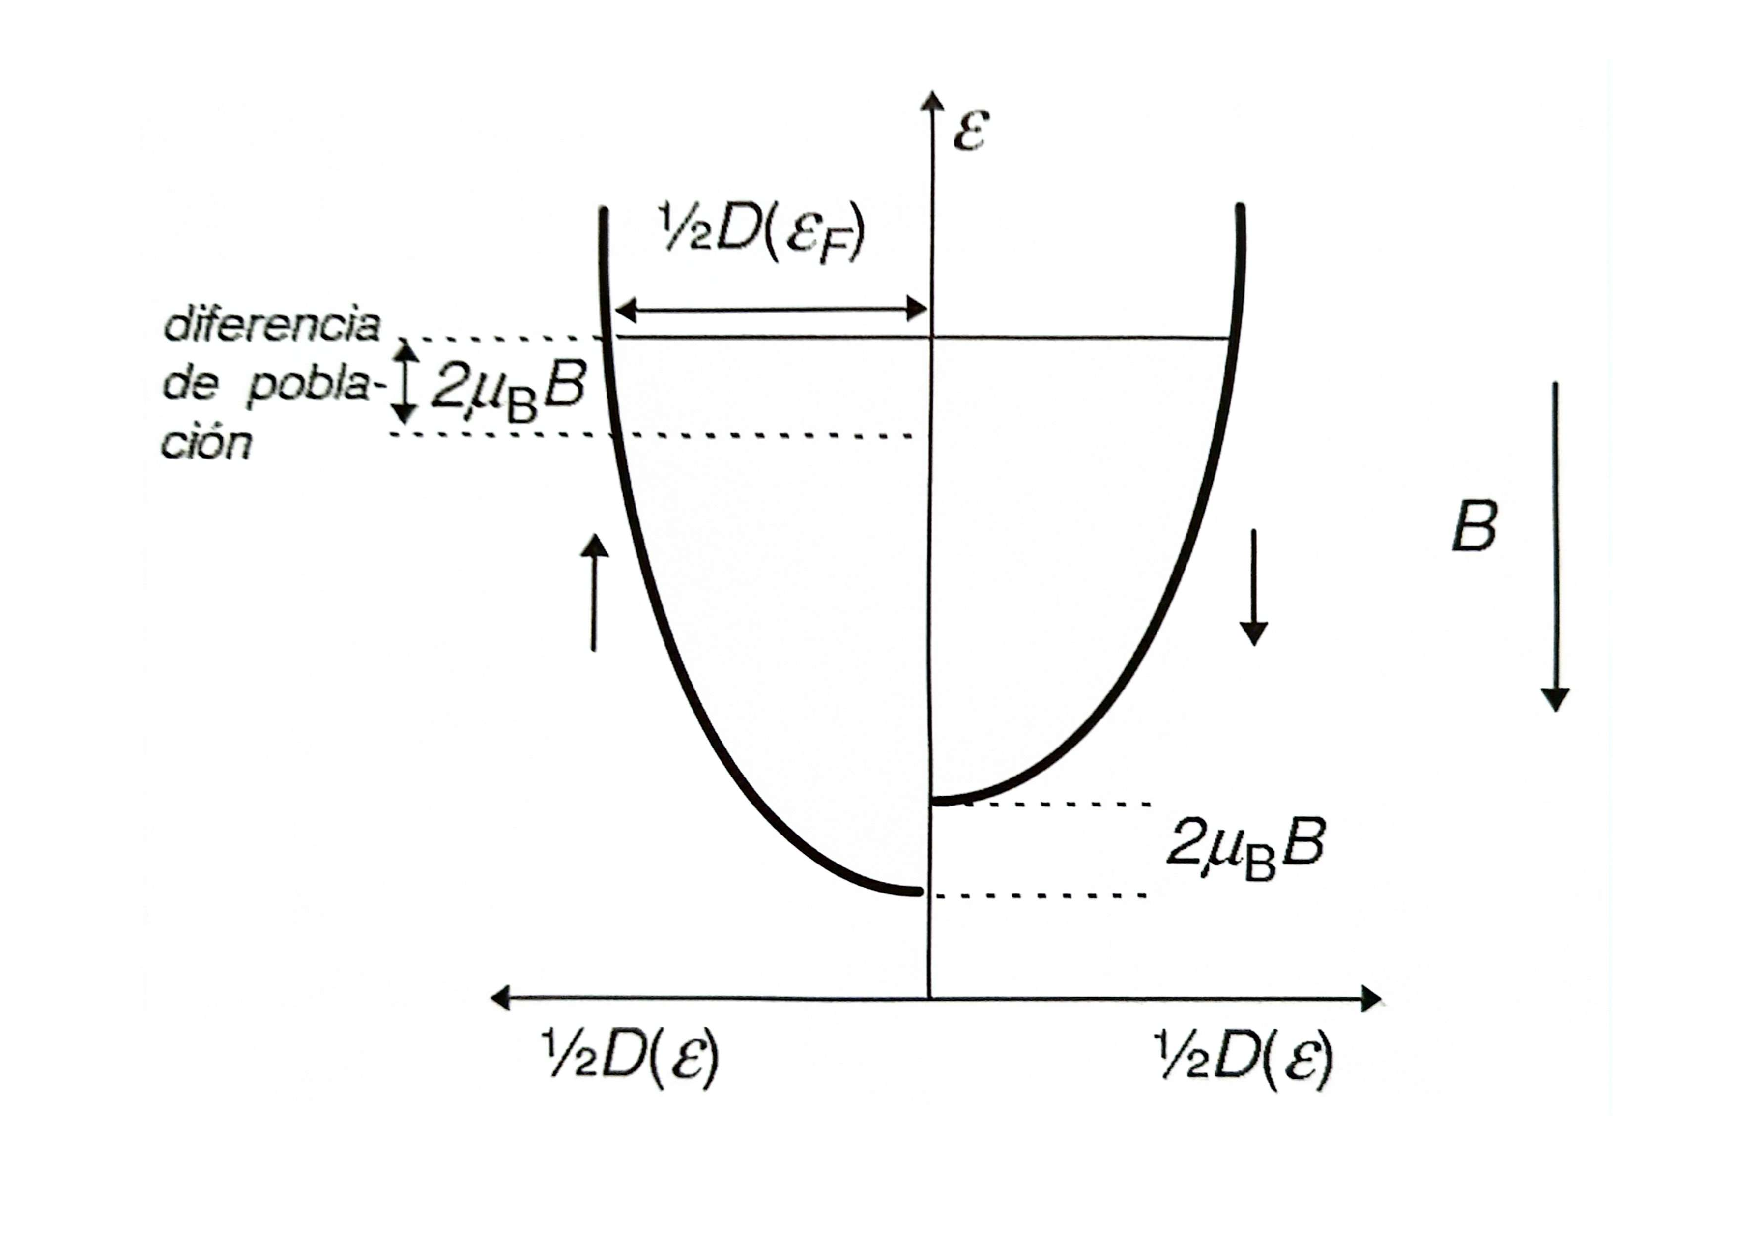
\includegraphics[scale=0.35]{Cuerpo/Ch_10/Fotos libro 3.pdf}
	\caption{Desplazamiento relativo de los niveles energéticos electrónicos correspondientes a espín $\uparrow$ y espín $\downarrow$.}
	\label{Fig:10-03}
\end{figure}
\begin{figure}[h!] \centering
	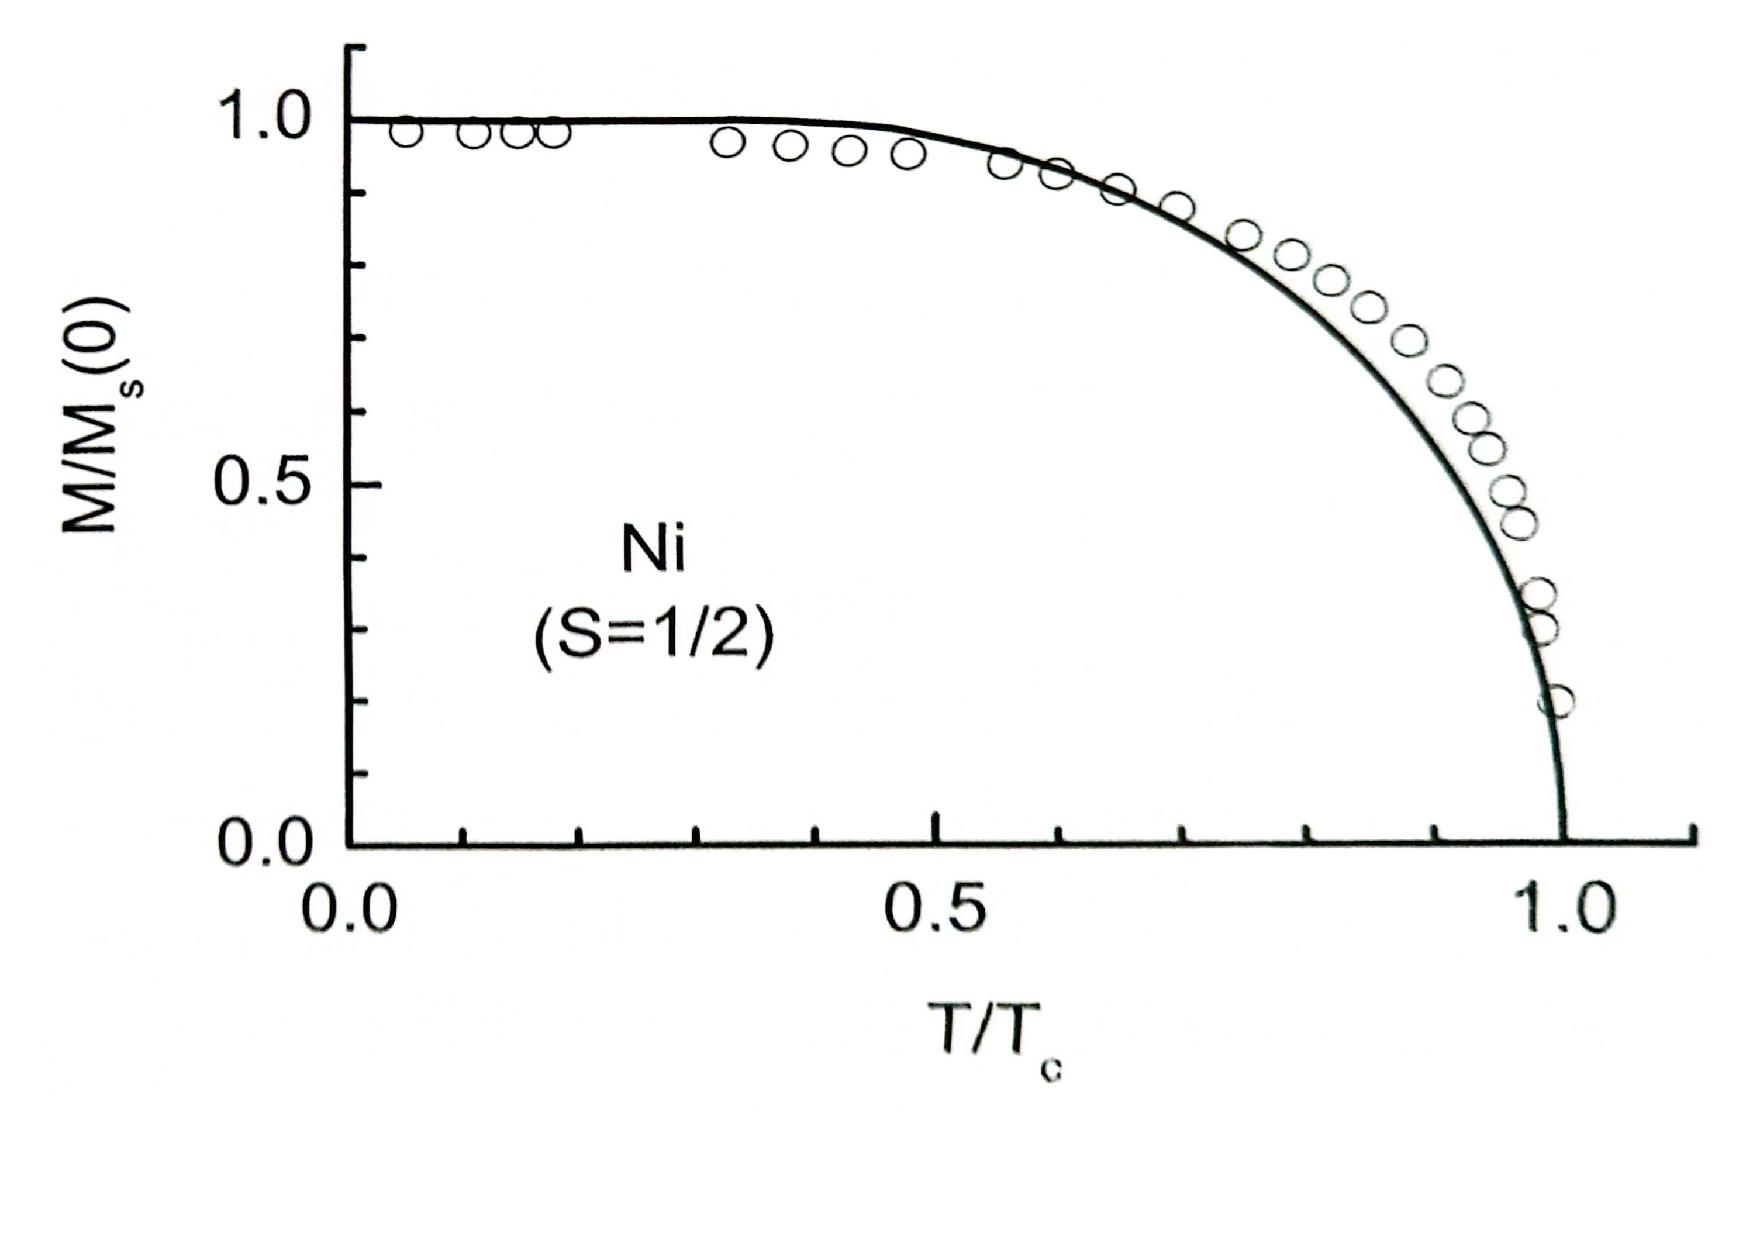
\includegraphics[scale=0.35]{Cuerpo/Ch_10/Fotos libro 4.pdf}
	\caption{Dependencia con la temperatura de la magnetización espontánea para el Ni cuando $T<T_C$, y compensación con las predicciones de campo medio.}
	\label{Fig:10-04}
\end{figure}
\begin{figure}[h!] \centering
	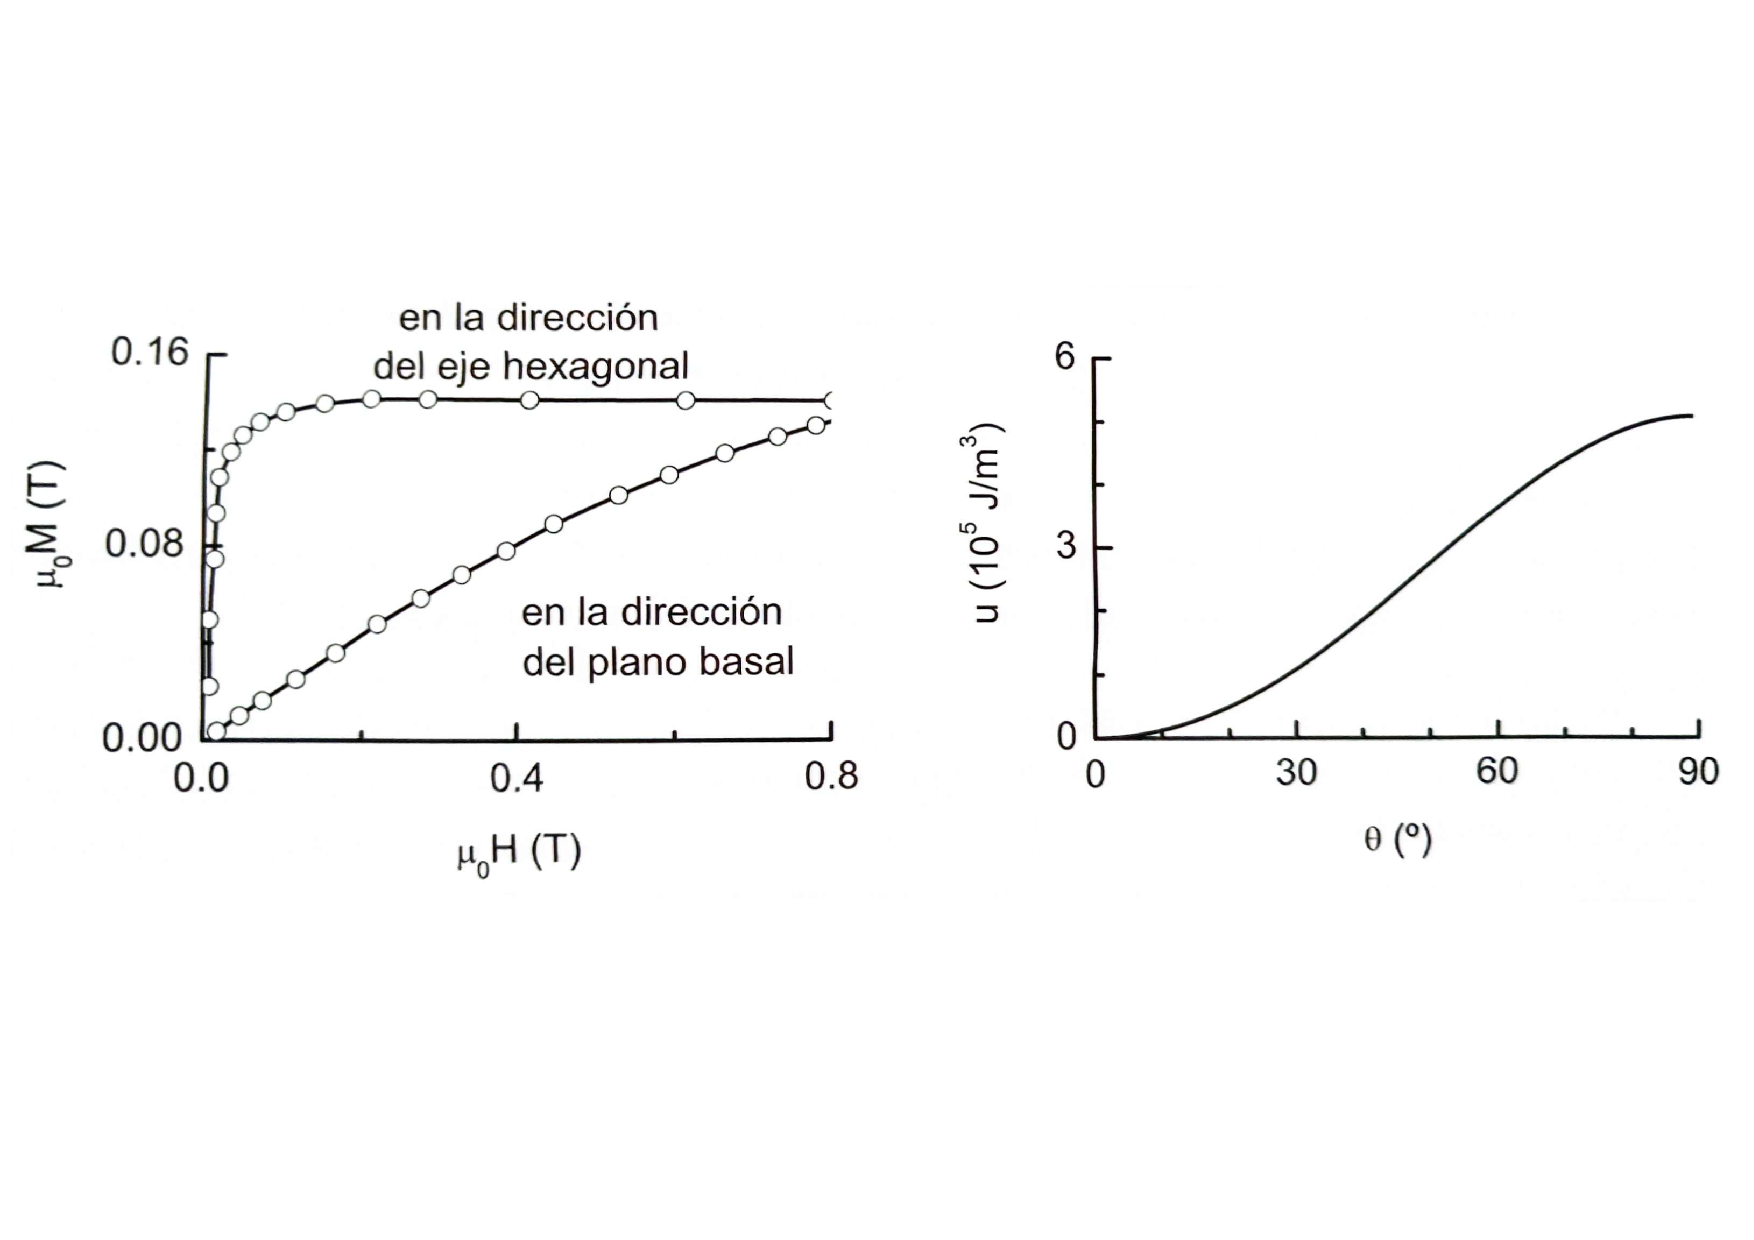
\includegraphics[scale=0.35]{Cuerpo/Ch_10/Fotos libro 5.pdf}
	\caption{En la izquierda la magnetización de una muestra de  Co para las direcciones paralela y perpendicular al plano basal de la estructura hexagonal. En la derecha de anisotropía del Co según el ángulo que forma la magnetización con el eje hexagonal.}
	\label{Fig:10-05}
\end{figure}
\begin{figure}[h!] \centering
	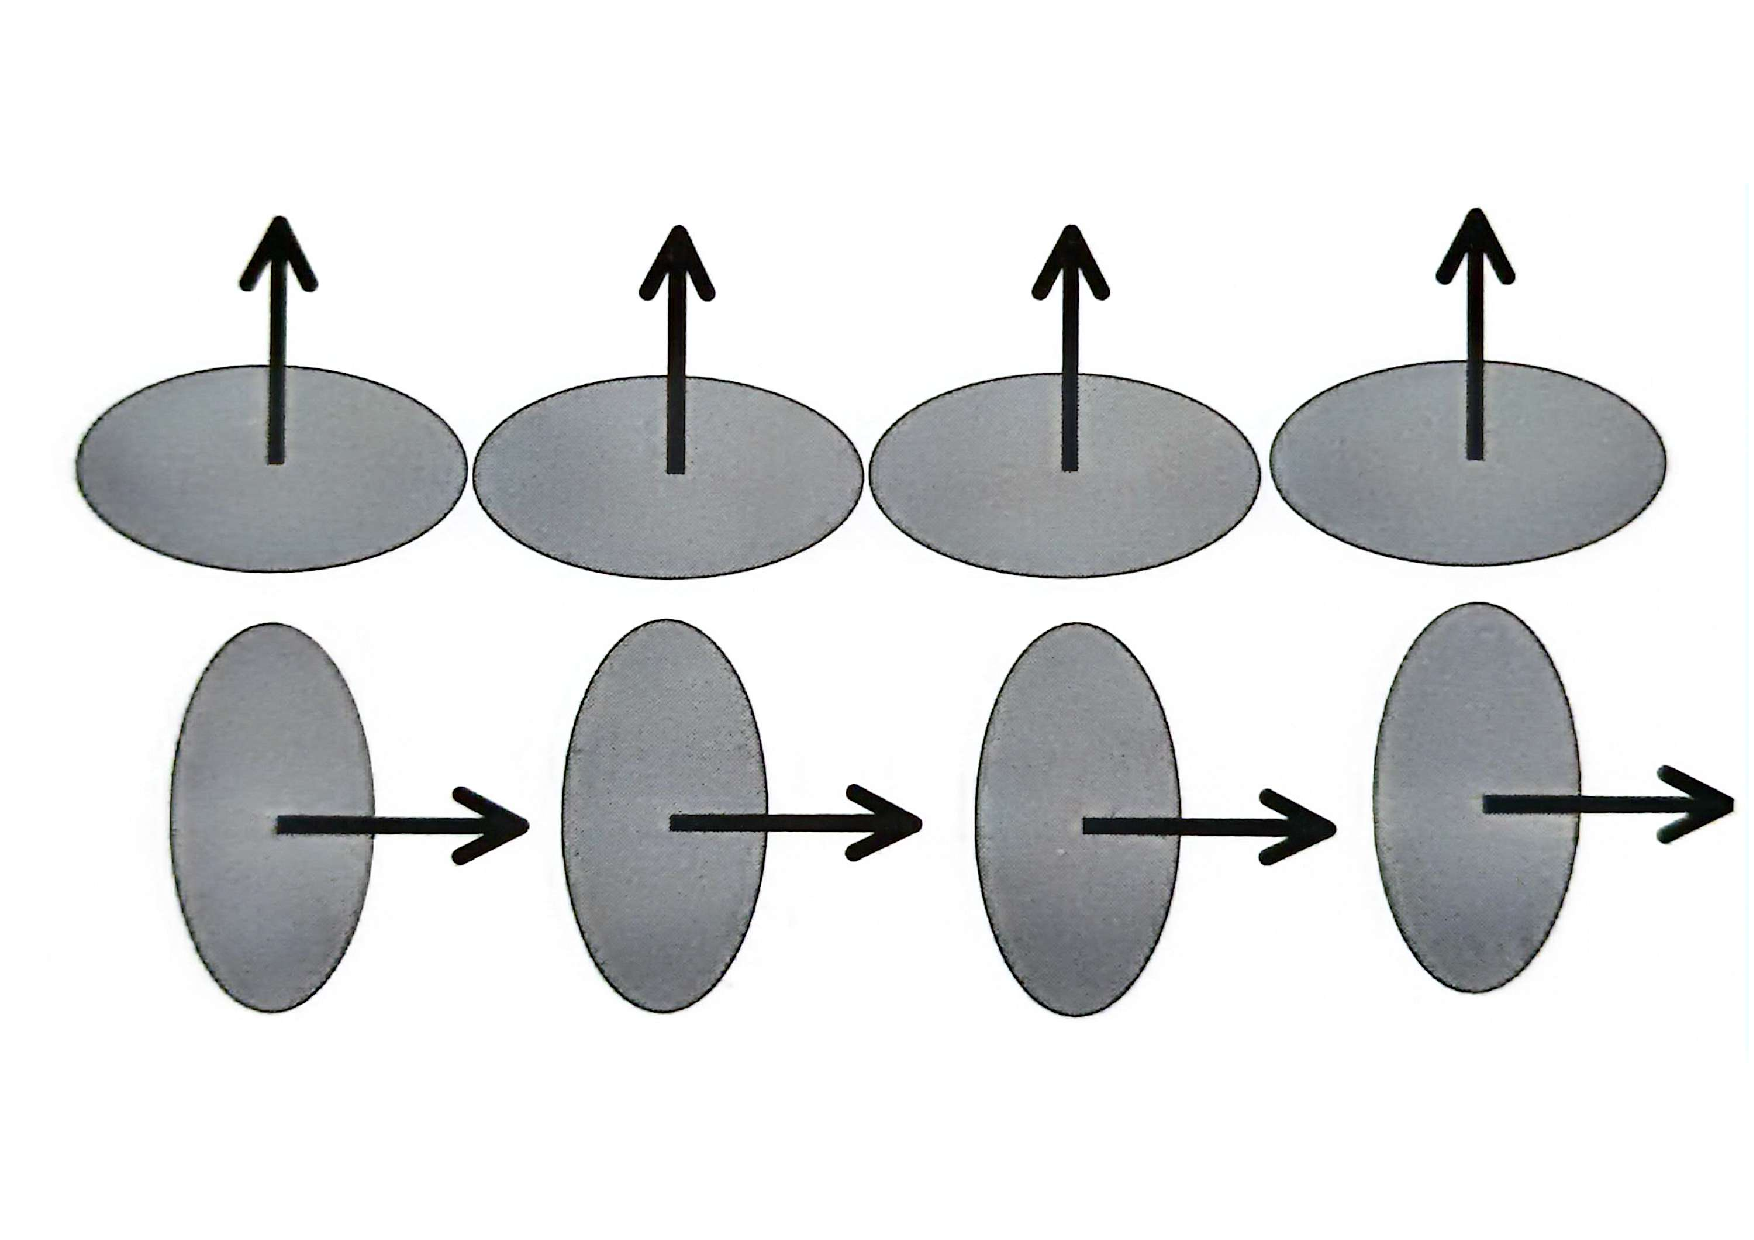
\includegraphics[scale=0.35]{Cuerpo/Ch_10/Fotos libro 6.pdf}
	\caption{Distribución electrónica para diferntes orientaciones del campo mangético aplicado.}
	\label{Fig:10-06}
\end{figure}
\begin{figure}[h!] \centering
	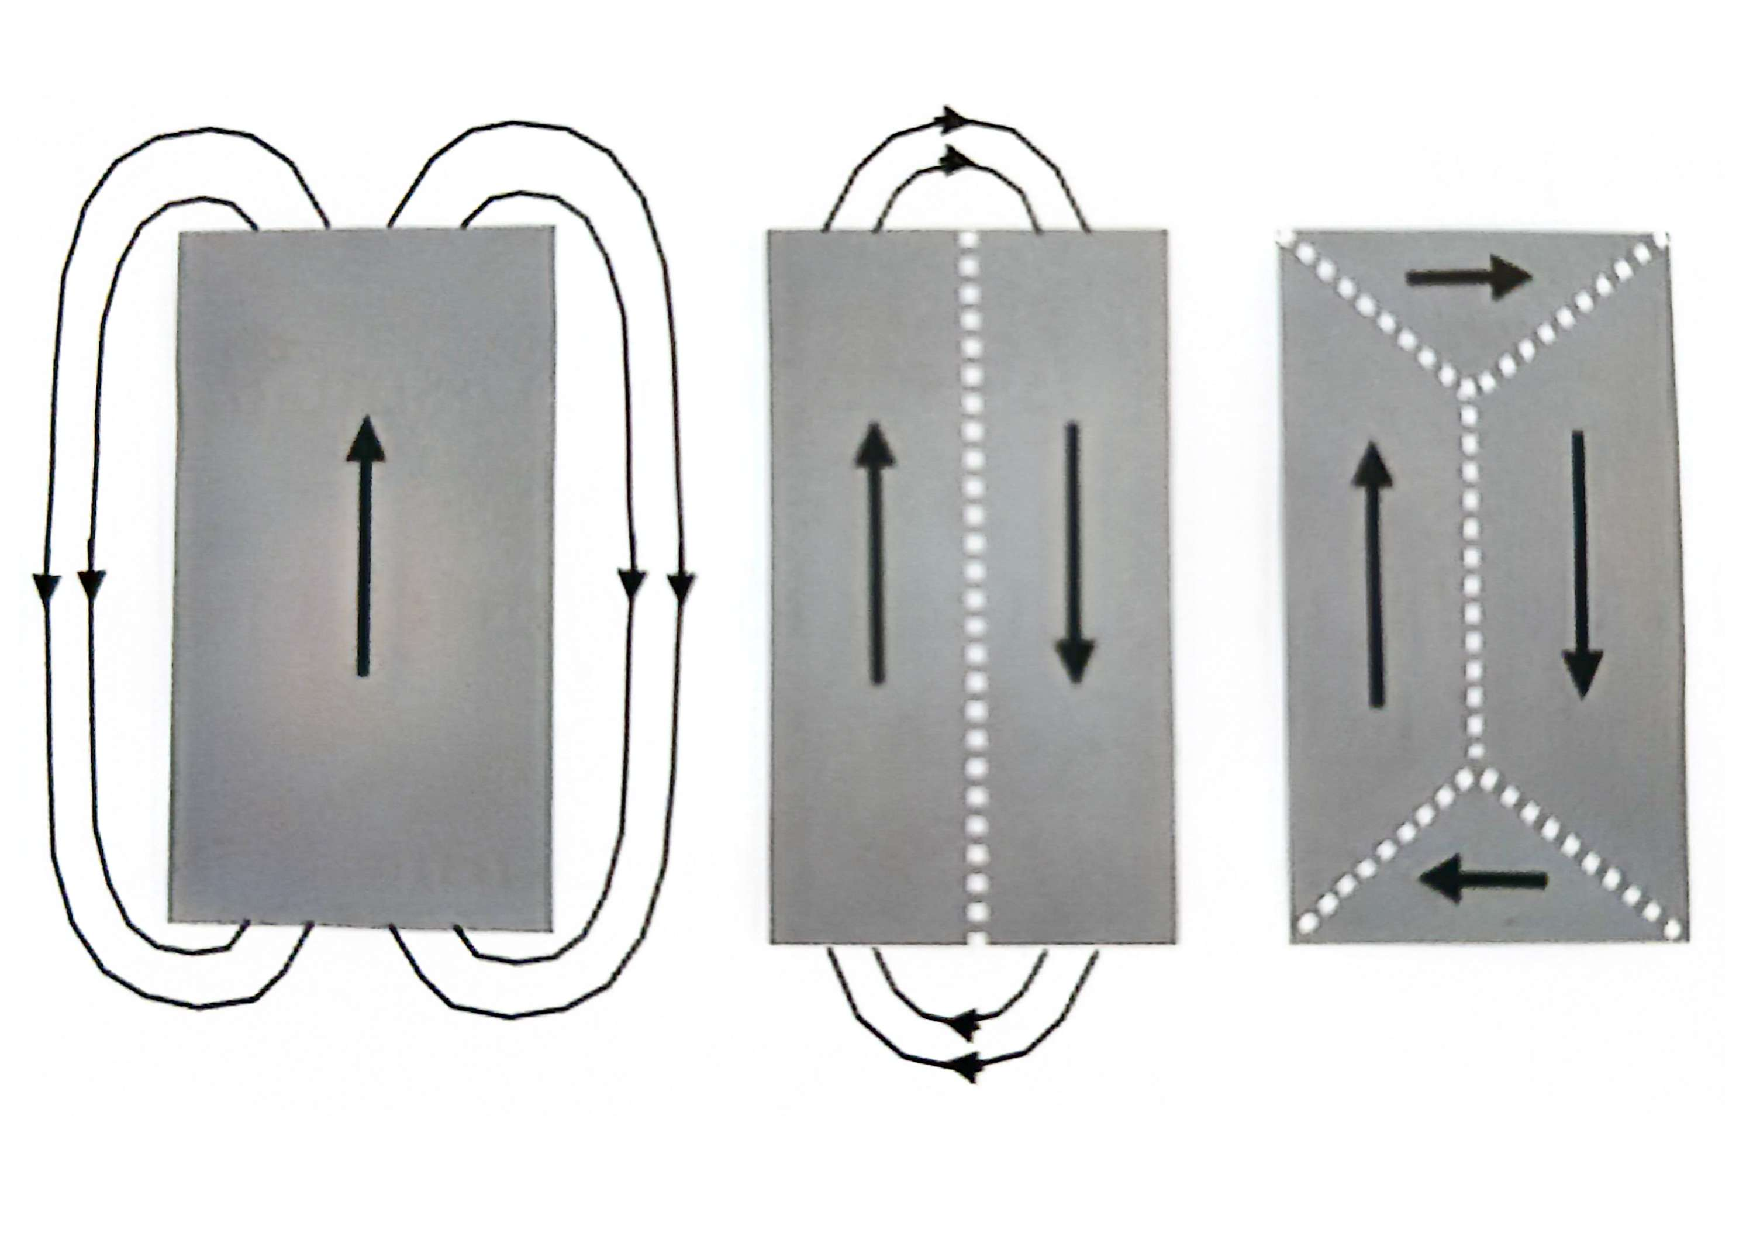
\includegraphics[scale=0.35]{Cuerpo/Ch_10/Fotos libro 7.pdf}
	\caption{Aparición de dominios en una muestra ferromagnética. Las flechas indican la orientación de los momentos magnéticos en cada dominio.}
	\label{Fig:10-07}
\end{figure}
\begin{figure}[h!] \centering
	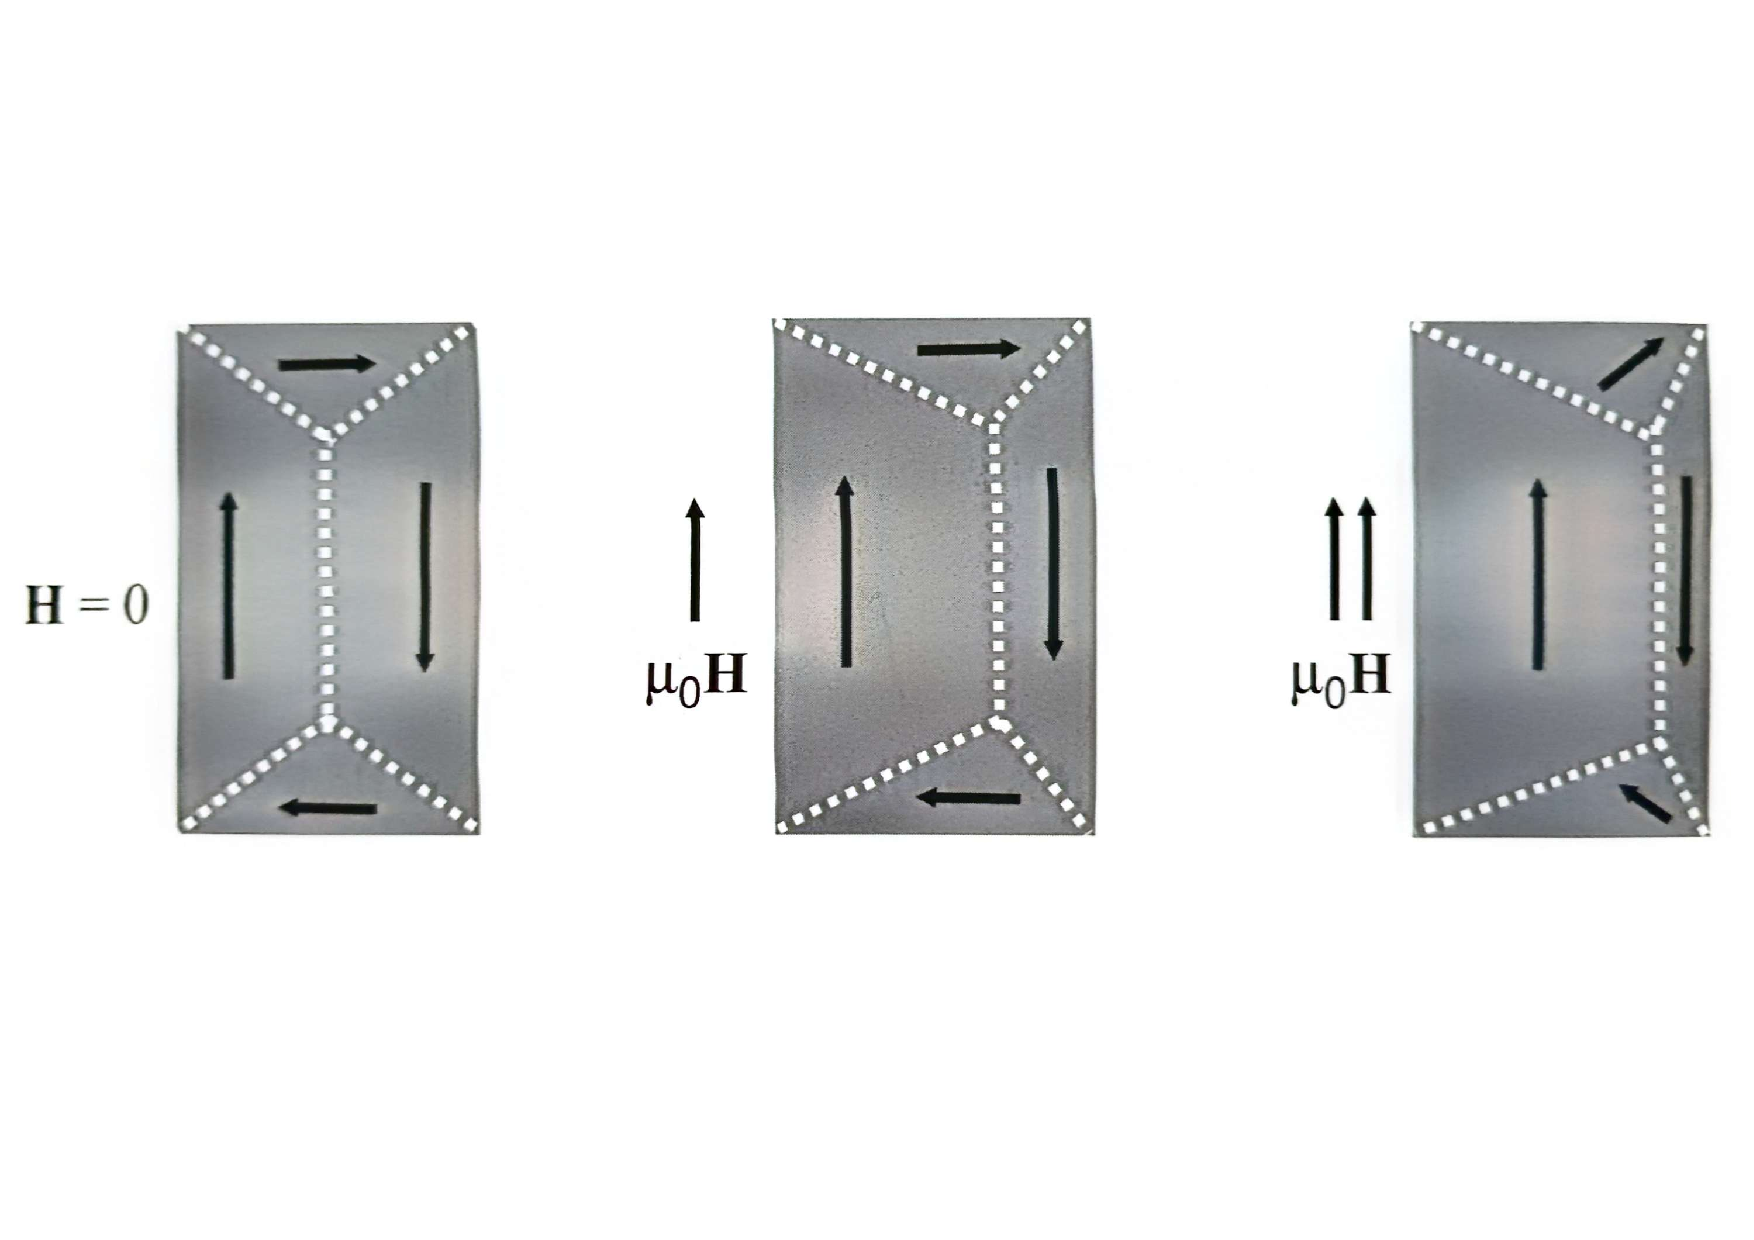
\includegraphics[scale=0.35]{Cuerpo/Ch_10/Fotos libro 8.pdf}
	\caption{Desplazamiento de las fronteras entre dominios debido a una variación del campo magnético aplicado.}
	\label{Fig:10-08}
\end{figure}
\begin{figure}[h!] \centering
	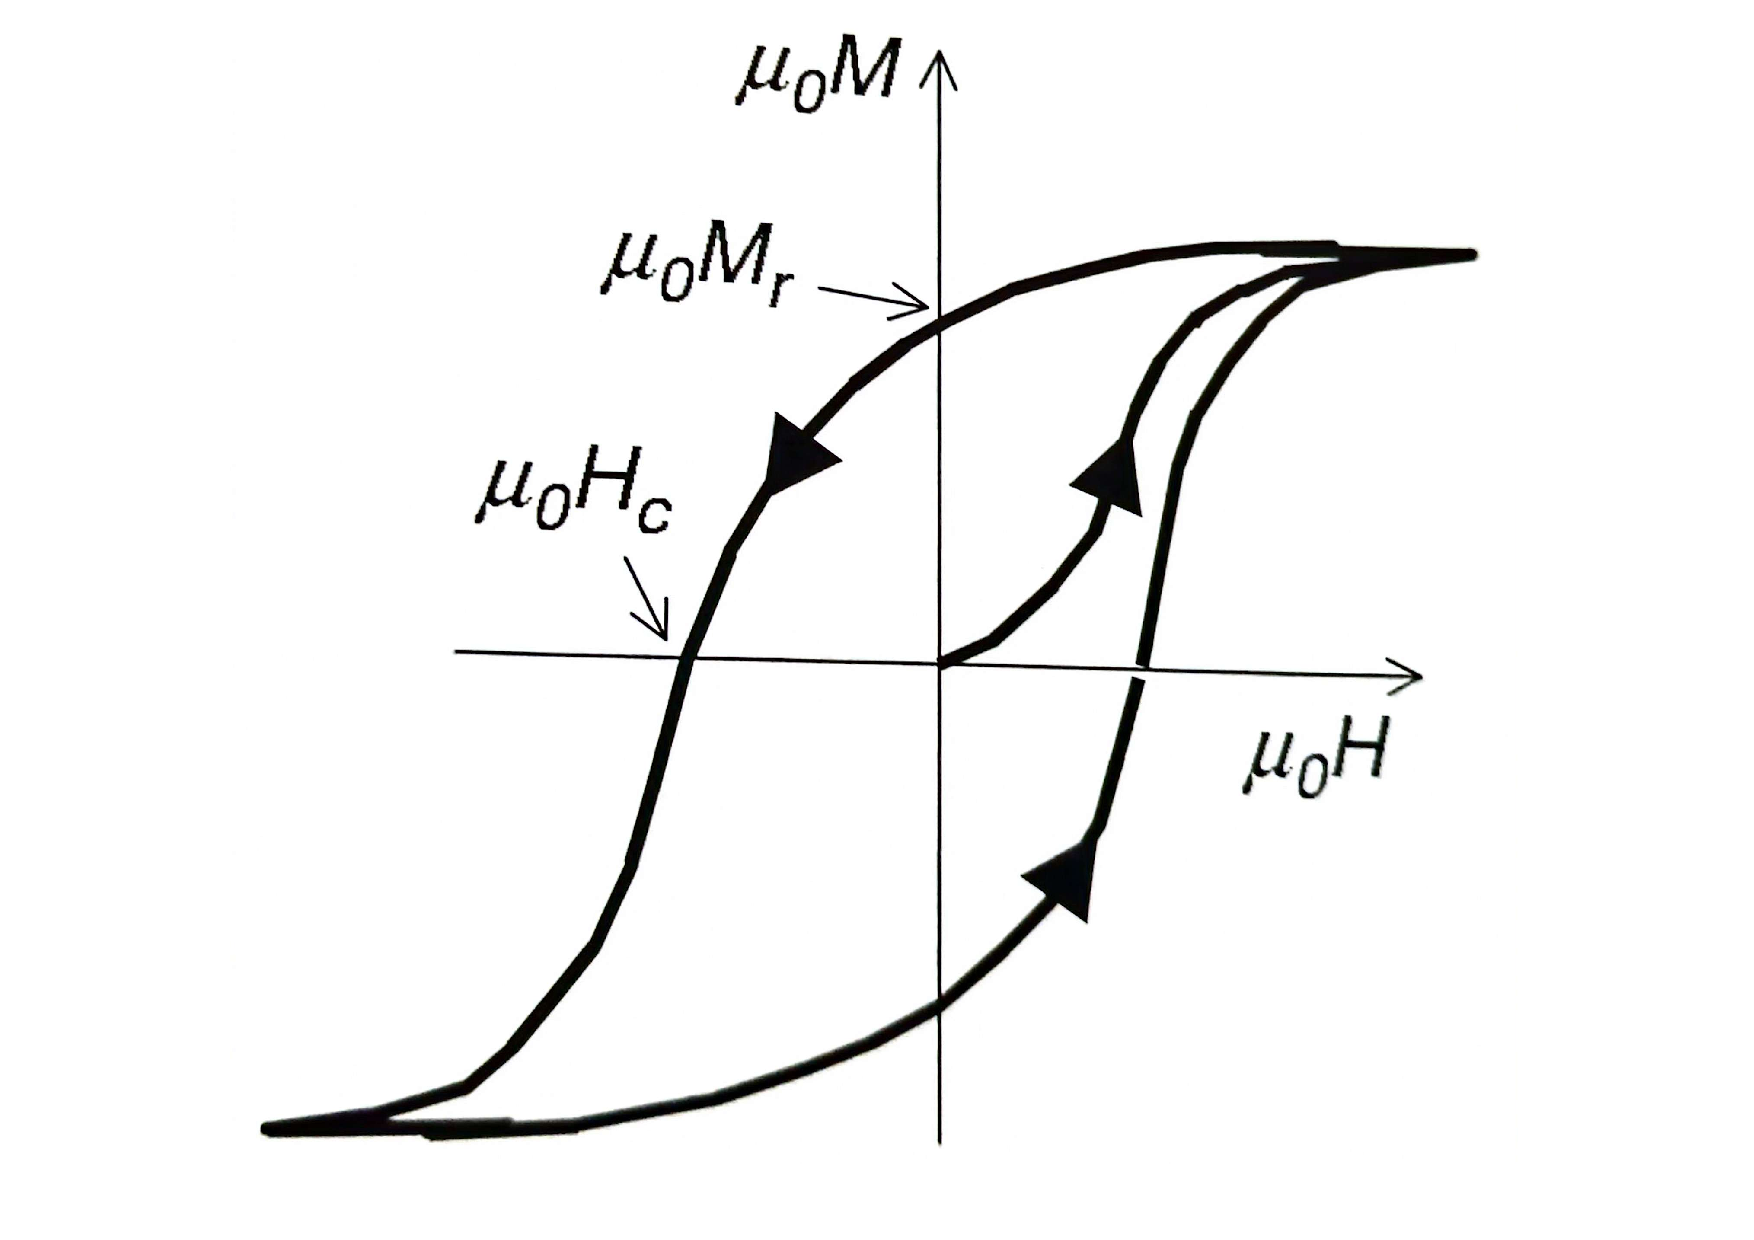
\includegraphics[scale=0.35]{Cuerpo/Ch_10/Fotos libro 9.pdf}
	\caption{Histéresis de la dependencia $M(H)$ debida al anclado de las paredes Bloch en los defectos del material.}
	\label{Fig:10-09}
\end{figure}